\chapter{Statistik und Wahrscheinlichkeiten}

\subsubsection{Literatur}

\begin{itemize}
	\item S.Brandt ,,Datenanalyse``
	\item G.Cowan ,,Statistical Data Analysis``
	\item R.Barlow ,,A Guide to the Use os Statistical Methods in Physical Sciences``
	\item F.James ,,Statistical and Computational Methods in Experimental Physics``
\end{itemize}
\folie{Einführung: Compass Experiment}\\
\folie{Einführung in die Statistik}

\section{Einführung}

2 mögliche Ansätze
\begin{enumerate}[a)]
	\item \textbf{Frequentist (Zählmensch) Axiome:}\\[10pt]
	Ereignismenge:
	\begin{equation*}
	E \defeq \left\{ \dots, A, B \right\}
	\end{equation*}
	\begin{enumerate}[1)]
		\item \begin{equation*}
		P(A) \ge 0 \quad \forall A \in E
		\end{equation*}
		\item \begin{equation*}
		\sum_{A \in E} P(A) = 1 \quad \Rightarrow \tx{ d.h.  \quad P(E) = 1}
		\end{equation*}
	\end{enumerate}
	wenn $ A_i $ tatsächlich Ereignisse sind, dann schließen sich $ A $ und $ B $ gegenseitig aus
	\begin{enumerate}[3)]
		\item \begin{equation*}
		P(A \land B) = P(A) + P(B)
		\end{equation*}
	\end{enumerate}
	nur gültig für den Fall $ A,B $ exklusiv
	\begin{equation*}
	\begin{aligned}
	\lor : \tx{oder} & \qquad \neg : \tx{nicht} \\
	\land : \tx{und} & \qquad \setminus : \tx{ohne}
	\end{aligned}
	\end{equation*}
	\begin{equation*}
	P(A \land \ol{A}) = P(A) + P(\ol{A}) = 1
	\end{equation*}
	\begin{equation*}
	\Rightarrow \quad 0 \le P(A) \le 1
	\end{equation*}
	\begin{figure}[ht]
		\centering
		%t1
		%\hft zwei mengen und schnittmenge
		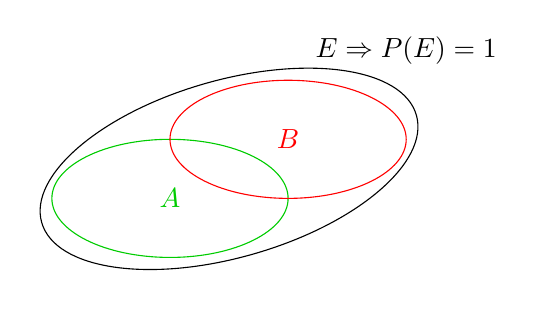
\begin{tikzpicture}[scale=0.75]
			\draw[green!80!black] (-1,-.5) ellipse (2cm and 1cm);
			\node[green!80!black] at (-1,-.5) {$ A $};
			\draw[red] (1,.5) ellipse (2cm and 1cm);
			\node[red] at (1,.5) {$ B $};
			\draw[rotate=16] (0,0) ellipse (3.3cm and 1.5cm);
			\node at (3,2) {$ E \Rightarrow P(E) = 1 $};
		\end{tikzpicture}
		\caption{Gesamtmenge $ E $ aller Ereignisse und zwei Ereinisse $ A, B \in E $.}
		\label{Mengen}
	\end{figure}
	\begin{align*}
	P(A + B + \dots) &= P(A) + P(B) + \dots \\
	P(\ol{A}) &= P(E \setminus A) = 1 - P(A) \\
	P(A \lor B) &= P(A) + P(B) - P(A \land B) \\
	P(A \land B) &= P(A) + P(B) - P(A \lor B) \\
	Ü(A \land B) + P(A \lor B) &= P(A) + P(B) \\
	\end{align*}
	\item \textbf{Bayes Statistik (bedingte Wahrscheinlichkeit)}\\[10pt]
	\begin{equation*}
	P(B|A) = \frac{P(A \land B)}{P(A)}
	\end{equation*}
	Allgemein:
	\begin{equation*}
	P(A|B) = \frac{P(B|A) \cdot P(A)}{\sum_i P(B|A_i) \cdot P(A_i)}
	\end{equation*}
	Beispielrechnung:\\
	Es gibt eine Krankheit und $ 0{,}1 \% $ der Bevölkerung sind erkrankt (Durchsendung). Es gibt einen Test um die Krankheit festzustellen mit einer $ 98\% $ Effizienz ($ \widehat{=} $ Gewissheit) und $ 3\% $ Fehlalarm ($ \widehat{=} $ Reinheit)\\[5pt]
	Frage: Was ist die Wahrscheinlichkeit erkrankt zu sein bei einem positiven Testergebnis (Befund) $ P(\tx{krank}|+) $
	\begin{align*}
	P(\tx{krank}) &= 0{,}001 \\
	P(\tx{gesund}) &= 0{,}999 \\
	P(+|\tx{krank}) &= 0{,}98 \\
	P(-|\tx{krank}) &= 0{,}02 \\
	\tx{Fehlalarm:} \quad P(+|\tx{gesund}) &= 0{,}03 \\
	P(-|\tx{gesund}) &= 0{,}97 \\
	\end{align*}
	\begin{align*}
	P(\tx{krank}|+) &= \frac{P(+|\tx{krang}) \cdot P(\tx{krank})}{P(+|\tx{krank}) \cdot P(\tx{krang}) + P(+|\tx{gesund}) \cdot P(\tx{gesund})} \\
	&= \frac{0{,}98 \cdot 0{,}001}{0{,}98 \cdot 0{,}001 + 0{,}03 \cdot 0{,}0999} = 0{,}032
	\end{align*}
	Die Wahrscheinlichkeit, bei einem positiven Testergebnis, krank zu sein ist also nur $ 3{,}2 \% $!!!
\end{enumerate}

\section{Verteilung einer Zufallsvariable}

\begin{description}
	\item[Population] Alle möglichen Eregnisse/Messungen
	\item[Stichprobenraum] Untermenge ausgewählter Stichproben
	\item[Zufallsvariable] \begin{itemize}
		\item diskret
		\item kontinuierlich
	\end{itemize}
	Verteilung einer Zufallsvariable $ x $ mit $ -\infty \le x \le + \infty $
\end{description}

Wahrscheinlichkeitsverteilung Beispiel: Würfel  $ P = \frac{1}{6} $


%T2
\hft Wkeit.vert. Würfel


\begin{equation*}
F(x) = \sum_{i=1}^{\tx{max}(x)} x p_i
\end{equation*}
monoton. $ \tx{max}(x) = $ ist der größte Wert für x.\\[10pt]
Wahrscheinlichkeitsdichte von $ x $
\begin{equation*}
f(x) = \prd{F}{x} = F'(x)
\end{equation*}
ist das Maß für die Wahrscheinlichkeit $ X $ eines Ereignisses $ X $
\begin{equation*}
x \le X \le x + \dd x
\end{equation*}

%T3
\hft
%T4
\hft


\folie{Histogrammdarstellung}

\subsection{Diskussion der Verteilungsfunktion}

\begin{enumerate}[a)]
	\item falls die Wahrscheinlichkeitsdichte differenzierbar ist\\
	$ \Rightarrow $ \textbf{Wahrscheinlichster Wert}
	\begin{equation*}
	\prd{}{x} f(x) = 0 \qquad \prd{^2}{x^2} f(x) < 0
	\end{equation*}
	\item \textbf{Median} $ x_{0.5} $ (50\% der Werte kleiner, 50\% der WErte größer)\\
	oder auch: Verteilungsfunktion hat den Wert; $ \frac{1}{2} $
	\begin{equation*}
	F(0.5) = P(X < x_{0.5})
	\end{equation*}
	\begin{equation*}
	\Rightarrow \quad \int_{-\infty}^{x_{0.5}} f(x) \dd x \overset{!}{=} 0.5
	\end{equation*}
	analog geht man vor für die Momente der Verteilung:
	\begin{equation*}
	E(x^n) = \int_{-\infty}^{\infty} x^n f(x) \dd x
	\end{equation*}
	hängt ab von der Wahrscheinlichkeitsdichteverteilung.\\[10pt]
	\textbf{Mittelwert (erstes Moment)}\\
	$ n = 1 $
	\begin{equation*}
	\mu = E(x) = \int_{-\infty}^{\infty} x f(x) \dd x
	\end{equation*}
	\textbf{Streuung um Mittelwert}
	\begin{equation*}
	E(x-\mu)^n = \int_{-\infty}^{\infty} (x-\mu)^n f(x) \dd x
	\end{equation*}
	um den Wahren Wert $ \mu $.\\[5pt]
	\textbf{Varianz}\\
	$ n = 2 $
	\begin{equation*}
	E(x-\mu)^2 = E(x^2) - \mu^2 = \int_{-\infty}^{\infty} f(x) \dd x
	\end{equation*}
	bei $ n = 3 $: Schiefe
\end{enumerate}

%03.06.19

\setcounter{section}{10}

\section{Wichtige Verteilungen}

\subsection*{Motivation}

Experiment + Theorie $ \to $ PDF $ f(N,\bar{E},w) $.

\subsection{Binomialverteilung}

Versuch mit zwei möglichen Ereignissen $ A $ und $ \bar{A} $ Z.B. Münzwurf. Die Wahrscheinlichkeiten dafür sind jeweils $ P(A) = p $ und $ P\bar{A} = 1 - p = q $. Bei $ N $ Wiederholungen des Versuchs ist die Wahrscheinlichkeit für 
\begin{equation*}
X = (\ub{A,A,A, \dots , A }_{n}, \ub{\bar{A},\bar{A},\bar{A}, \dots, \bar{A}}_{N - n})
\end{equation*}
gleich
\begin{equation*}
P(X) = p^n \cdot q^{N-n}
\end{equation*}
Diese Ereignisse können an
\begin{equation*}
\begin{pmatrix}
N \\ n
\end{pmatrix} = \frac{N!}{n! (N-n)!}
\end{equation*}
auftreten.
\begin{equation*}
B = f(n,N,p) = \begin{pmatrix}
N \\ n
\end{pmatrix} p^n q^{N-n}
\end{equation*}
mit der Anzahl des Auftretens von $ A $ als Laufparameter $ n \in \mathbb{N}_{0} $.\\[10pt]

\subsubsection{Erwartungswert}

\begin{equation*}
E(B(N,p)) = \sum_{n=0}^{N} n \begin{pmatrix}
N \\ n
\end{pmatrix} p^n q^{N-n} = \dots = N \cdot p
\end{equation*}
Summenregel für Erwartungswerte
\begin{equation*}
E[X_1+ \dots + X_N] = E[X_1] + E[X_2] + \dots + E[X_N] = N E[X_1] = N \cdot p
\end{equation*}

\subsubsection{Varianz}

\begin{equation*}
V[n] = E[n^2] - E[n]^2 = N \cdot p (1 - p) = N p q
\end{equation*}
Beispiel 1: Münzwurf wird übersprungen.\\[5pt]
\textbf{Beispiel 2: 10 Exp Messungen einer Größe}\\[10pt]
Fehler mit $ p = 0{,}683 $ liegt der Wahre Wert in dem Intervall $ [x, \pm \sigma] $
\begin{equation*}
B(10,10,0{,}683) = 0{,}683^{10} \approx 0{,}02
\end{equation*}
Man würde also erwarten, dass die Fehler überschätzt wurden.

\subsection{Poisson Verteilung}

Beschreibt im Wesentlichen die Binomialverteilung im Grenzfall für $ N \to \infty $ und $ p \to 0 $. $ \Rightarrow \ N \cdot p = \nu $ endlich.
\begin{equation*}
B(n, N, p) \to f(n,\nu) = \frac{\nu^n}{n!} e^{-\nu}
\end{equation*}

\subsubsection{Erwartungswert}

\begin{equation*}
E[n] =\sum_{n=0}^{\infty} n \cdot \frac{\nu^n}{n!} \cdot e^{-\nu} = \sum_{n=1}^{\infty} n \cdot \frac{\nu^n}{n!} \cdot e^{-\nu} = \nu e^{-\nu} \ub{\sum_{n=1}^{\infty} \frac{\nu^{n-1}}{(n-1)!}}_{e^{\nu}} = \nu
\end{equation*}

\subsubsection{Varianz}

\begin{equation*}
V[n] = \sum_{n=0}^{\infty} (n-\nu)^2 \frac{\nu^n}{n!} e^{-\nu} = \nu
\end{equation*}
Standartabweichung $ \sigma = \sqrt{\nu} $\\[5pt]
\textbf{Beispiel 3: 50 Szintillatoren 1 Jahr Messen}\\[10pt]
\begin{equation*}
P(A) = 0{,}01 = 1\%
\end{equation*}
Wobei $ A \widehat{=} $ Szintillator kaputt nach $ \le 1 $ Jahr
\begin{equation*}
\tx{Binomial :} \quad B(0,50,0{,}01) = \begin{pmatrix}
50 \\ 0
\end{pmatrix} 0{,}01^{0} \cdot 0{,}93^{50} = 0{,}067
\end{equation*}
\begin{equation*}
\tx{Poisson :} \quad f(0,0{,}5) = e^{-0{,}5} = 0{,}607
\end{equation*}
$ \nu = N \cdot p = 0{,}5 $

\subsection{Gleichverteilung}

\begin{equation*}
f(x; \alpha, \beta) = \casess{\frac{1}{\beta - \alpha}}{\alpha \le x \le \beta}{0}{\tx{sonst}}
\end{equation*}
Erwartungswert und Varianz:
\begin{align*}
E[x] &= \frac{1}{2} (\alpha + \beta) \\
V[x] &= \frac{1}{12} (\beta - \alpha)^2
\end{align*}

\subsection{Gauß-Verteilung / Normalverteilung}

\emph{Definition} einer Wahrscheinlichkeitsdichte:
\begin{enumerate}[1.]
	\item $ f(x) \ge 0 \ \forall x $
	\item $ f(x) $ muss integrierbar sein.
	\item $ \int_{-\infty}^{\infty} f(x) \dd x = 1 $
\end{enumerate}
\begin{equation*}
f(x;\mu,\sigma^2) = \frac{1}{\sqrt{2 \pi \sigma^2}} e^{\frac{-(x-\mu)^2}{2 \sigma^2}}
\end{equation*}
2 Parameter:
\begin{itemize}
	\item $ \mu = $ Mittelwert
	\item $ \sigma =  $ Standartabweichung
\end{itemize}

\subsubsection{Erwartungswert}

\begin{equation*}
E[X] = \int_{-\infty}^{\infty} x \cdot f(x; \mu, \sigma^2) \dd x = \dots = \mu
\end{equation*}

\subsubsection{Varianz}

\begin{equation*}
V[X] = \int_{-\infty}^{\infty} (x - \mu)^2 \cdot f(x; \mu, \sigma^2) = \dots = \sigma^2
\end{equation*}

\begin{equation*}
\tx{Verteilungs Dichte (PDF)} \overset{\tx{Integration}}{\longrightarrow} \tx{Verteilungsfunktion (CDF)}
\end{equation*}
Oft betrachtet man die Standard Normalverteilung:
\begin{equation*}
\mu = 0 \qquad \sigma = 1
\end{equation*}
\begin{equation*}
x = \frac{x}{\sigma} - \mu
\end{equation*}
\begin{equation*}
\Phi(x) = \frac{1}{\sqrt{2 \pi}} \int_{-\infty}^{\infty} e^{\frac{1}{2} t^2} \dd t
\end{equation*}
Verteilungsfunktion der Standard Normalverteilung

